\newpage
\section[Day 8: Open Relative and Compact]
{Closure, Open Relative, \& Compact}

\subsection{ Closure }

{ \color{blue} Definition 8.1.1: Closure } 

	\begin{adjustbox}{minipage=14cm, right, vspace=0.1cm 0cm}
        Let E $\subset$ metric space X and E' be the set of all
        limit points of E in X.

        \qquad Then the closure of E:
            \qquad $\overline{E}$ = E $\cup$ E'

        with the properties:
	\end{adjustbox}

	\begin{enumerate}[label=(\alph*), leftmargin=2cm, itemsep=0.1cm]
        \item $\overline{E}$ is closed
        
        \item E = $\overline{E}$ if and only if E is closed
        
        \item $\overline{E}$ $\subset$ F for every closed F $\subset$ X
        such that E $\subset$ F
    \end{enumerate}

{ \color{magenta} \underline{Proof} } 

	Suppose x $\in$ X, but x $\not \in$ $\overline{E}$. Thus, x $\in$ $\overline{E}^c$.

	Thus, there is a N$_r(x)$ $\subset$ $\overline{E}^c$ since else there is
	always a p $\in$ N$_r(x)$ where p $\in$ $\overline{E}$ so x is a limit point
	of $\overline{E}$ so x $\in$ $\overline{E}$.
	Thus, $\overline{E}^c$ is open so $\overline{E}$ is closed by
	{\color{red} theorem 7.1.7}.

	\vspace{0.2cm}

	If E = $\overline{E}$, then by part (a), E is closed.

	If E is closed, then E' $\subset$ E so E = E $\cup_{}^{}$ E' = $\overline{E}$.

	\vspace{0.2cm}

	If closed set F, then F' $\subset$ F and since E $\subset$ F, then
	E' $\subset$ F' $\subset$ F.
	Thus, $\overline{E}$ $\subset$ F. \\

{ \color{red} Theorem 8.1.2: sup(E) $\in$ $\overline{E}$ }

    \begin{adjustbox}{minipage=14cm, right, vspace=0.1cm 0cm}
        Let non-empty set of real numbers, E, be bounded above.
        
        Let y = sup(E). Then, y $\in$ $\overline{E}$.
        Thus, y $\in$ E if E is closed.
    \end{adjustbox}

{ \color{magenta} \underline{Proof} } 
	
	If y $\in$ E, then y $\in$ $\overline{E}$. Suppose y $\not \in$ E.

	For every h $>$ 0, there exists a x $\in$ E such that y-h $<$ x $<$ y
	otherwise y-h is an upper bound for E which is a contradiction
	since y = sup(E).

	Thus, y is a limit point of E so y $\in$ $\overline{E}$.





\subsection{ Open Relative }

{ \color{blue} Definition 8.2.1: Open Relative }

	\begin{adjustbox}{minipage=14cm, right, vspace=0.1cm 0cm}
		Suppose E $\subset$ Y $\subset$ metric space X.

		Then E is open relative to Y if for each p $\in$ E, there is an
		r $>$ 0

		such that for any q $\in$ Y, then q $\in$ E if d(q,p) $<$ r. \\
	\end{adjustbox}

{ \color{red} Theorem 8.2.2: E is open relative to Y $\subset$ X
if E = Y $\cap$ G and G is open in X} 

	\begin{adjustbox}{minipage=14cm, right, vspace=0.1cm 0cm}
		Suppose E $\subset$ Y $\subset$ X.

		E is open relative to Y if and only if E = Y $\cap$ G
		for some open G $\subset$ X.
	\end{adjustbox}

{ \color{magenta} \underline{Proof}: } 

	Suppose E is open relative to Y.

	Then for each p $\in$ E, there is a r$_p$ $>$ 0 such that for
	any q $\in$ Y where d(p,q) $<$ r$_p$, then q $\in$ E.
	
	Since Y $\subset$ X, let V$_p$ be the set of all q $\in$ X
	such that d(p,q) $<$ r$_p$ and define G = $\cup_{p \in E}^{}$ V$_p$.
	Since V$_p$ is open by {\color{red} theorem 7.1.3}, then by
	{\color{red} theorem 7.1.9a}, open G $\subset$ X.

	Since p $\in$ V$_p$ for all p $\in$ E, then E $\subset$ G $\cap_{}^{}$ Y.
	Also, by construction, then V$_p$ $\cap_{}^{}$ Y $\subset$ E so
	G $\cap_{}^{}$ Y $\subset$ E.
	Thus, E = Y $\cap_{}^{}$ G.

	If G is open in X and E = G $\cap_{}^{}$ Y, then every p $\in$ E has
	a V$_p$ $\subset$ G.

	Then, V$_p$ $\cap_{}^{}$ Y $\subset$ G $\cap_{}^{}$ Y = E so E is open relative to Y.
\newpage	





\subsection{ Compact Sets }

{ \color{blue} Definition 8.3.1: Open Cover } 

	\begin{adjustbox}{minipage=14cm, right, vspace=0.1cm 0cm}
		An open cover of set E $\subset$ X is a collection of open $G_1, G_2, ...$
		$\subset$ X
		
		such that E $\subset$ $\cup_{}^{}$ $G_i$. \\
	\end{adjustbox}

{ \color{blue} Definition 8.3.2: Compact } 

	\begin{adjustbox}{minipage=14cm, right, vspace=0.1cm 0cm}
		K $\subset$ X is compact if every open cover
		of K contains a finite subcover.

		\qquad If $G_1, G_2, ...$ is an open cover of K, then
		K $\subset$ $\cup_{i=1}^{n}$ $G_i$ for some n. \\
	\end{adjustbox}

{ \color{red} Theorem 8.3.3: A compact set is compact in every metric space } 

	\begin{adjustbox}{minipage=14cm, right, vspace=0.1cm 0cm}
		Suppose K $\subset$ Y $\subset$ X.

		Then K is compact relative to X if and only if K is
		compact relative to Y.
	\end{adjustbox}

{ \color{magenta} \underline{Proof} } 

	Suppose K is compact relative to X.

	Let $V_1, V_2, ...$ be sets open relative to Y such that
	K $\subset$ $\cup_{}^{}$ $V_x$.
	Then by {\color{red} theorem 8.2.2} for each $V_x$, there is a
	$G_x$ open relative to X where $V_x$ = Y $\cap_{}^{}$ $G_x$.

	Since K is compact relative to X, then there is a n such that
	K $\subset$ $G_{x_1}$ $\cup_{}^{}$ ... $\cup_{}^{}$ $G_{x_n}$.

	Thus, K = K $\cap_{}^{}$ Y $\subset$ ($\cup_{i=1}^{n}$ $G_{x_i}$) $\cap_{}^{}$ Y
	= ($\cup_{i=1}^{n}$ $G_{x_i}$ $\cap_{}^{}$ Y) = $\cup_{i=1}^{n}$ $V_{x_i}$.
	
	Since there are open $V_{x_1}, ... , V_{x_n}$ where
	K $\subset$ $\cup_{i=1}^{n}$ $V_{x_i}$ so K is compact relative to Y.

	Suppose K is compact relative to Y.

	Let open $G_1, G_2, ...$ $\subset$ X such that X $\subset$ $\cup_{}^{}$ $G_x$.
	For each $G_x$, let $V_x$ = Y $\cap_{}^{}$ $G_x$ $\subset$ Y.

	Since K is compact relative to Y, there is a n such that
	K $\subset$ $\cup_{i=1}^{n}$ $V_{x_i}$.

	Thus, K $\subset$ $\cup_{i=1}^{n}$ $V_{x_i}$
	= $\cup_{i=1}^{n}$ (Y $\cap_{}^{}$ $G_{x_i}$)
	$\subset$ $\cup_{i=1}^{n}$ $G_{x_i}$ so K is compact relative to X.

\begin{figure}[h]
	\centering
	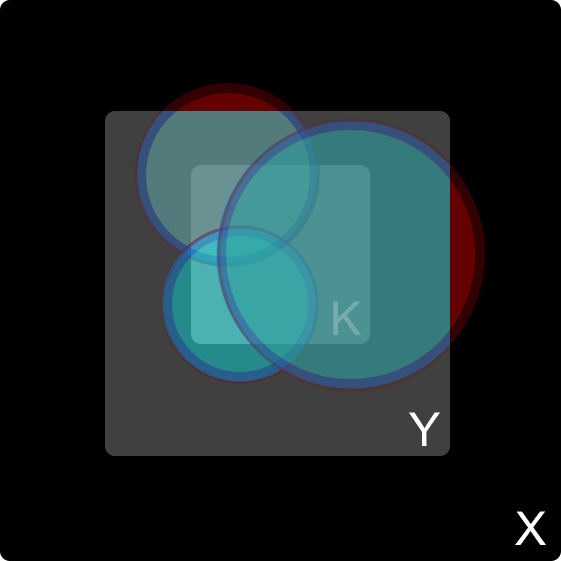
\includegraphics[scale=0.35]{Images/8.3.3.png}
\end{figure}

{ \color{red} Theorem 8.3.4: A compact set is closed } 

	\begin{adjustbox}{minipage=14cm, right, vspace=0.1cm 0cm}
		Compact subsets of metric spaces are closed.
	\end{adjustbox}

{ \color{magenta} \underline{Proof} } 

	Let compact K $\subset$ X.
	Suppose p $\in$ X, but p $\not \in$ K so p $\in$ K$^c$.

	If q $\in$ K, let W$_q$ be a neighborhood of q with
	r $<$ $\frac{1}{2}$d(p,q).
	Let V$_{p,q}$ be a neighbohood of p with r $<$ $\frac{1}{2}$d(p,q).
	Since K is compact, then there are finite points $q_1, ... , q_n$
	such that K $\subset$ W where W = W$_{q_1}$ $\cup$ ... $\cup$ W$_{q_n}$.

	Let V = V$_{p,q_1}$ $\cap$ ... $\cap$ V$_{p,q_n}$, then
	K $\cap$ V $\subset$ W $\cap$ V = $\emptyset$ so V $\subset$ K$^c$.

	Since there is a neighborhood V for p $\in$ K$^c$ where V $\subset$ K$^c$,
	then every p $\in$ K$^c$ is an interior point so K$^c$ is open.
	Then by {\color{red} theorem 7.1.7}, K is closed. \\

\newpage

\begin{figure}[h]
	\centering
	
\includegraphics[scale=0.35]{Images/8.3.4.png}
\end{figure}

{ \color{red} Theorem 8.3.5: If closed E $\subset$ compact set K, E is compact } 

	\begin{adjustbox}{minipage=14cm, right, vspace=0.1cm 0cm}
		Closed subsets of compact sets are compact.
	\end{adjustbox}

{ \color{magenta} \underline{Proof} } 

	Suppose F $\subset$ K $\subset$ X where F is closed relative to X
	and K is compact.

	Let $V_1, V_2, ...$ be an open cover for F.
	Let open set F$^c$ be all k $\in$ K where k $\not \in$ F.

	\qquad K = F $\cup$ F$^c$ $\subset$ $V_1$ $\cup$ $V_2$ $\cup$ ... $\cup$ F$^c$

	Thus, $V_1$ $\cup$ $V_2$ $\cup$ ... $\cup$ F$^c$ is an open cover for K.

	Since K is compact, there is a finite subcover $\Omega$ that covers K
	and thus, finite subcover $\Omega$ covers F $\cup$ F$^c$.
	
	Remove F$^c$ from $\Omega$. Since finite subcover $\Omega$ - F$^c$ covers F,
	then F is compact. \\

{ \color{orange} Corollary 8.3.6: Closed F $\cap$ compact K = compact } 

	\begin{adjustbox}{minipage=14cm, right, vspace=0.1cm 0cm}
		If F is closed and K is compact, then F $\cap_{}^{}$ K is compact.
	\end{adjustbox}

{ \color{magenta} \underline{Proof} } 

	Since K is compact, then K is closed by {\color{red} theorem 8.3.4}.

	Then, by {\color{red} 7.1.9b}, F $\cap$ K is closed.

	Since F $\cap$ K $\subset$ K, then by {\color{red} theorem 8.3.5},
	F $\cap$ K is compact. \\

{ \color{red} Theorem 8.3.7: Nonempty $\cap_{i=1}^n$ $K_i$ $\rightarrow$
nonempty $\cap$ $K_i$ } 

	\begin{adjustbox}{minipage=14cm, right, vspace=0.1cm 0cm}
		For compact sets $K_1, K_2, ...$ $\subset$ X where any intersection
		of finite $K_i$ is nonempty, then $\cap$ $K_i$ is nonempty.
	\end{adjustbox}

{ \color{magenta} \underline{Proof} } 

	Fix $K_1$.
	If there is a k $\in$ $K_1$ where k $\in$ $K_i$ for all i, then
	k $\in$ $\cap$ $K_i$ so $\cap$ $K_i$ $\not =$ $\emptyset$.

	Suppose for every k $\in$ $K_1$, k $\not \in$ $K_i$ for some i.

	Then for every k $\in$ $K_1$, there is a $K_i$ such that
	p $\not \in$ $K_i$ so p $\in$ $K_i^c$.

	Thus, $K_2^c, k_3^c, ...$ form an open cover for $K_1$.

	Since $K_1$ is compact, there is a n where
	$K_1$ $\subset$ $K_{i_1}^c$ $\cup$ ... $\cup$ $K_{i_n}^c$.

	But then, $K_1$ $\cap$ $K_{i_1}$ $\cap$ ... $\cap$ $K_{i_n}$
	= $\emptyset$ which is a contradiction. \\

{ \color{orange} Corollary 8.3.8: Nonempty $K_i$ where $K_{i+1}$ $\subset$ $K_i$
$\rightarrow$ nonempty $\cap$ $K_i$}

	\begin{adjustbox}{minipage=14cm, right, vspace=0.1cm 0cm}
		If $K_1, K_2, ...$ is a sequence of nonempty compact sets
		such that $K_{i+1}$ $\subset$ $K_i$, then $\cap$ $K_i$ is nonempty.
	\end{adjustbox}

{ \color{magenta} \underline{Proof} } 

	Since each $K_i$ is nonempty and if $i_1 < ... < i_n$, then
	$K_{i_1}$ $\cap$ ... $\cap$ $K_{i_n}$
	= $K_{i_n}$ is nonempty, then
	by {\color{red} theorem 8.3.7}, $\cap$ $K_i$ is nonempty. \\

\newpage

{ \color{red} Theorem 8.3.9: Nonempty intervals $I_n$ where
$I_{n+1}$ $\subset$ $I_n$ $\rightarrow$ nonempty $\cap$ $I_n$}

	\begin{adjustbox}{minipage=14cm, right, vspace=0.1cm 0cm}
		If $I_1, I_2, ...$ is a sequence of intervals in $\mathbb{R}^1$
		such that $I_{n+1}$ $\subset$ $I_n$,
		
		then $\cap$ $I_n$ is nonempty.
	\end{adjustbox}

{ \color{magenta} \underline{Proof} } 

	Let $I_n$ = [$a_n$,$b_n$] and thus, each $I_n$ is nonempty.
	If $n_1 < ... < n_m$, then

	$I_{n_1}$ $\cap$ ... $\cap$ $I_{n_m}$
	= [$a_{n_m}$,$b_{n_m}$] is nonempty.
	Thus, by {\color{red} theorem 8.3.7}, $\cap$ $I_n$ is nonempty. \\

{ \color{red} Theorem 8.3.10: p $\in$ E' exists if
infinite E $\subset$ compact K }

	\begin{adjustbox}{minipage=14cm, right, vspace=0.1cm 0cm}
		If E is an infinite subset of compact set K, then E has a
		limit point in K.
	\end{adjustbox}

{ \color{magenta} \underline{Proof} } 

	If no p $\in$ K is a p $\in$ E', then each p would have
	a neighbohood $V_p$ contains at most p $\in$ E if p $\in$ E.
	Thus, there is no finite subcover that covers E and thus,
	there is no finite subcover that covers K since E $\subset$ K
	which contradicts K is compact. \\

{ \color{red} Theorem 8.3.11: Heine-Borel Theorem } 

	\begin{adjustbox}{minipage=14cm, right, vspace=0.1cm 0cm}
		If a set E $\subset$ $\mathbb{R}^k$ has one of the three properties,
		then it has the other two:
	\end{adjustbox}

	\begin{enumerate}[label=(\alph*), leftmargin=2cm, itemsep=0.1cm]
		\item E is closed and bounded
		\item E is compact
		\item Every infinite subset of E has a limit point in E
	\end{enumerate}

{ \color{magenta} \underline{Proof} } 

	Suppose E is closed and bounded.

	Then there exists a M $\in$ $\mathbb{R}$ and q $\in$ $\mathbb{R}^k$
	such that d(p,q) $<$ M for all p $\in$ E.
	
	Thus, there is a k-cell
	K = [$-M+q_1$,$q_1+M$] $\times$ ... $\times$ [$-M+q_k$,$q_k+M$]
	such that E $\subset$ K.

	Since K $\subset$ $N_{\sqrt{kM^2}}(q)$, then K is compact
	and thus by {\color{red} theorem 8.3.5}, E is compact
	so (a) $\rightarrow$ (b).

	Then by {\color{red} thereom 8.3.10}, any infinite subset
	of E has a limit point in E so (b) $\rightarrow$ (c).

	Suppose E is not bounded.

	Then there exists p $\in$ E such that d(p,q) $>$ M for
	any M $\in$ $\mathbb{R}$ and q $\in$ $\mathbb{R}^k$.

	Let S $\subset$ E be such points p.
	
	Then S is infinite else there is a maximal p and thus,
	p is bounded.
	Thus, S is infinite and contains no limit points in E
	since any d($p_1$,$p_2$) $>$ M which contradicts that
	every infinite subset of E has a limit point in E.
	Thus, E is bounded.

	Suppose E is not closed.

	Then there exists a p $\in$ E', but p $\not \in$ E.
	Since p is a limit point, then there is a
	q $\in$ E such that $\frac{1}{n+1}$ $<$ d(q,p) $<$ $\frac{1}{n}$
	for n = \{1, 2, ...\}.

	Let S $\subset$ E be such points q.

	Thus, p is the only limit point of S since for r $<$ $\frac{1}{n}$,
	any N$_r(q_i)$ contains no points of S other than $q_i$ since
	d($q_i$,$q_j$) $>$ $\frac{1}{n}$ for any $q_1$,$q_2$ $\in$ S.
	
	Thus, S is infinite, but the only p $\in$ S' is p $\not \in$ E
	which contradicts that every infinite subset of E has a
	limit point in E. Thus, E is closed. So, (c) $\rightarrow$ (a). \\

{ \color{red} Theorem 8.3.12: Weierstrass Theorem } 

	\begin{adjustbox}{minipage=14cm, right, vspace=0.1cm 0cm}
		Every bounded infinite set E $\subset$ $\mathbb{R}^k$ has
		a limit point in $\mathbb{R}^k$.
	\end{adjustbox}

{ \color{magenta} \underline{Proof} } 

	Since E is bounded, then there exists a k-cell K such that
	E $\subset$ K.
	Since K is compact, then by {\color{red} theorem 8.3.10},
	E has a limit point in K and thus, in $\mathbb{R}^k$.





